\section{alamSYS System Tests Results and Discussions}
\label{sec:alamSYS_res}
With the development of alamSYS, we must ensure that all of its components 
are functioning properly. This section focuses on the system's 
performance while idle and under load, as well as the API's and 
database's ability to handle multiple requests at a time.
\\

The Table \ref{tab:idle_sys_utilization} shows the CPU and memory
utilization of each of the alamSYS components whenever it is not
processing any information. Wherein, the data presented below
is gathered by logging the system utilization of alamSYS within
an hour.
\\

% tab:idle_sys_utilization
\begin{longtable}[c]{cccc}
    \caption{Idle System Average Resource Usage Statistics}
    \label{tab:idle_sys_utilization}\\
    \hline
                                                                                & \textbf{alamAPI} & \textbf{alamDB} & \textbf{alamPREPROCESSOR} \\ \hline
    \endfirsthead
    %
    \multicolumn{4}{c}%
    {{\bfseries Table \thetable\ continued from previous page}} \\
    \hline
                                                                                & \textbf{alamAPI} & \textbf{alamDB} & \textbf{alamPREPROCESSOR} \\ \hline
    \endhead
    %
    \textbf{\begin{tabular}[c]{@{}c@{}}CPU\\ Utilization (\%)\end{tabular}}     & 0.168125         & 0.254313        & 0.009769                  \\
    \textbf{\begin{tabular}[c]{@{}c@{}}Memory\\ Utilization (MiB)\end{tabular}} & 45.718311        & 166.775377      & 312.798300                \\ \hline
\end{longtable}}
From the table above, it is shown that the alamSYS as a whole
only utilizes 0.432207\% of the total CPU power on average
when it is on idle. Wherein, the bulk of the CPU power is
being used by the database at 0.254313\% which is 58.84\%
of the total average CPU utilization of the alamSYS.
\\

This result actually shows promising idle performance, as an Ubuntu system's 
normal idle CPU utilization is less than 10\%. However, it should be noted 
that the alamSYS is not completely idle because background tasks such as 
scheduling, mongoDB processes, and the API must remain active in order to 
respond to any API queries.
\\

Furthermore, the lower average CPU utilization for alamAPI and 
alamPREPROCESSOR could be attributed to the linux distribution 
used as their base image, as previously discussed on 
'Docker-Compose Layer Diagram' of Section \ref{sec:system_diagrams}.
\\

The CPU utilization for the alamPREPROCESSOR, in particular, was 
lower than we would have expected given that it is running a schedule 
checker every second. This indicate that the schedule library utilizes
an efficient way to check for schedules. However, it may not be the case
for its memory utilization, which is discussed further below.
\\

Moving on, the alamSYS's memory utilization shows that it uses 
525.291988 Mebibytes (MiB) or 550.808572 Megabytes (MB) on average. 
The memory utilization of alamPREPROCESSOR accounts for the majority 
(59.55\%). This demonstrates that, despite having the lowest CPU 
utilization, the alamPREPROCESSOR consumes more memory than the 
combination of the alamAPI and alamDB.
\\

Again, as previously discussed, the alamPREPROCESSOR's high 
average memory utilization is due to the background schedule 
checking, which in this case is programmed to use more memory 
than CPU power.
\\

This average utilization result implies that the alamSYS may 
be able to be deployed on devices with lower specifications. 
A Raspberry Pi 4, which has a quad core CPU and at least 2GB RAM, 
is one example \cite{Zwetsloot2019}. However, idle performance only shows the minimum CPU 
and memory utilization of the alamSYS components and does not 
provide a complete picture of its utilization, particularly under 
load. As a result, we must investigate the system's CPU and memory 
utilization while under load.
\\

The internal load averages system utilization of the alamSYS' preprocessor 
is shown in the following table.
\\

% tab:intenal_load_stats
\begin{longtable}[c]{cccc}
    \caption{Internal Load Average Resource Usage Statistics}
    \label{tab:intenal_load_stats}\\
    \hline
    \multicolumn{1}{l}{}                                                                 & \textbf{Data Collector} & \textbf{Data Processor} & \textbf{\begin{tabular}[c]{@{}c@{}}alamSYS\\ PREPROCESSOR\\ (Data Collector \\ \& Data Processor)\end{tabular}} \\ \hline
    \endfirsthead
    %
    \multicolumn{4}{c}%
    {{\bfseries Table \thetable\ continued from previous page}} \\
    \hline
    \multicolumn{1}{l}{}                                                                 & \textbf{Data Collector} & \textbf{Data Processor} & \textbf{\begin{tabular}[c]{@{}c@{}}alamSYS\\ PREPROCESSOR\\ (Data Collector \\ \& Data Processor)\end{tabular}} \\ \hline
    \endhead
    %
    \hline
    \endfoot
    %
    \endlastfoot
    %
    \textbf{\begin{tabular}[c]{@{}c@{}}Failure Rate \\ (\%)\end{tabular}}                & 0                       & 0                       & 0                                                                                                               \\
    \textbf{\begin{tabular}[c]{@{}c@{}}Success Rate \\ (\%)\end{tabular}}                & 100                     & 100                     & 100                                                                                                             \\
    \textbf{\begin{tabular}[c]{@{}c@{}}Average Runtime\\ (s)\end{tabular}}               & 41.72398                & 8.38061                 & 48.30466                                                                                                        \\
    \textbf{\begin{tabular}[c]{@{}c@{}}Average CPU\\ Utilization (\%)\end{tabular}}      & 11.40659                & 92.71117                & 20.03138                                                                                                        \\
    \textbf{\begin{tabular}[c]{@{}c@{}}Average Memory\\ Utilization (MiB)\end{tabular}}  & 3.64200                 & 57.09545                & 794.29436                                                                                                       \\
    \textbf{\begin{tabular}[c]{@{}c@{}}Average Network \\ Utilization (Mb)\end{tabular}} & 232.73640               & 154                     & 77.27655                                                                                                        \\ \hline
\end{longtable}}
Before exploring into the results shown in Table \ref{tab:intenal_load_stats}, 
it is critical to first establish a context for how the data was gathered. 
The data in the above table was collected while the alamSYS, specifically the 
alamPREPROCESSOR, was subjected to a stress test load of 100 consecutive 
data collection and processing. Also, the data of average utilization as 
indicated for each column are independently gathered from each other.
\\

Based on the table above, each component was capable of processing 100 
consecutive processes without failure. This means that the alamSYS, 
specifically the alamPREPROCESSOR, can run at least 100 times in a row without 
ailing. Also, keep in mind that the alamPREPROCESSOR only collects and 
processes data once per day, and the developer has included an option for 
system users or maintainers to manually rerun these processes in cases where 
the alamPREPROCESSOR fails - for example, due to a lost or slow internet 
connection, a power outage, and so on.
\\

Meanwhile, the data processor's average runtime is faster than the data 
collector's, and it runs on an average of 48.30466 seconds. This was already 
expected because the data collector needed to connect to the internet and was 
thus constrained by internet speed. Whereas the average speed during the 
course of this test was 52.98Mbps, this could imply that the data collector's 
runtime may be slower or faster depending on the internet speed.
\\

Furthermore, the data processor's average runtime was surprisingly fast given 
that it needed to apply DMD-LSTM to a total of 20 stocks and calculate the 
position using the ALMACD given a total of 205 data points. Furthermore, 
looking at its CPU and memory utilization, it can be seen that it uses more 
than the data collector, with approximately 87.68\% more average CPU power 
used and approximately 93.63\% more average memory used.
\\

In line with the CPU and memory utilization, the average CPU utilization 
of the alamPREPROCESSOR on load is 99.95\% higher than when it is idle. 
And it uses 60.62\% more memory on average.
\\

Lastly, looking at the network utilization of the alamPREPROCESSOR, we can see 
that the data collector used the most network bandwidth, as expected. However, 
it may be surprising to see that the data processor uses the network when it 
should not because it does not need to process or collect data from the 
internet, but this is still within expectations because network bandwidth 
utilization also accounts for local network utilization. The data processor 
of alamPREPROCESSOR, in particular, uses the local network to connect to and 
update the new data in the alamDB.
\\

The following tables show the system's deployment load results. 
Specifically, to access the buy and sell collections, as shown 
in Tables \ref{tab:buy_reqs} and \ref{tab:sell_reqs}. Additionally, 
to have a background on the test that results in the following 
outcomes. It should be noted that the test consisted of three 
instances of the same tester application running on ten different 
computers. Where each application requests 10, 100, 1000 buy and 
sell data from the alamDB via the alamAPI, which is tunneled over 
the internet for server access outside the university's local 
network using LocalXpose services.
\\

% tab:buy_reqs
\begin{longtable}[c]{cccc}
    \caption{Deployment Load Test Results (Buy Requests)}
    \label{tab:buy_reqs}\\
    \hline
                                                                                   & \multicolumn{3}{c}{\textbf{Number or Requests}} \\
    \endfirsthead
    %
    \multicolumn{4}{c}%
    {{\bfseries Table \thetable\ continued from previous page}} \\
    \hline
                                                                                   & \multicolumn{3}{c}{\textbf{Number or Requests}} \\
    \endhead
    %
    \hline
    \endfoot
    %
    \endlastfoot
    %
                                                                                   & \textbf{10}   & \textbf{100}   & \textbf{1000}  \\ \hline
    \textbf{\begin{tabular}[c]{@{}c@{}}Success Rate\\ (\%)\end{tabular}}           & 100           & 100            & 100            \\
    \textbf{\begin{tabular}[c]{@{}c@{}}Average Processing\\ Time (s)\end{tabular}} & 11.905222     & 139.618550     & 1159.773569    \\ \hline
\end{longtable}}

% tab:sell_reqs
\begin{longtable}[c]{cccc}
    \caption{Deployment Load Test Results (Sell Requests)}
    \label{tab:sell_reqs}\\
    \hline
                                                                                   & \multicolumn{3}{c}{\textbf{Number or Requests}} \\
    \endfirsthead
    %
    \multicolumn{4}{c}%
    {{\bfseries Table \thetable\ continued from previous page}} \\
    \hline
                                                                                   & \multicolumn{3}{c}{\textbf{Number or Requests}} \\
    \endhead
    %
    \hline
    \endfoot
    %
    \endlastfoot
    %
                                                                                   & \textbf{10}   & \textbf{100}   & \textbf{1000}  \\ \hline
    \textbf{\begin{tabular}[c]{@{}c@{}}Success Rate\\ (\%)\end{tabular}}           & 100           & 100            & 100            \\
    \textbf{\begin{tabular}[c]{@{}c@{}}Average Processing\\ Time (s)\end{tabular}} & 13.384126     & 130.119867     & 1642.995011    \\ \hline
\end{longtable}}
As per the tables above, the alamSYS was able to handle all 
consecutive and simultaneous requests from all external devices. 
It was able to handle 71,000 requests in approximately one hour 
and 20 minutes.
\\

Furthermore, the data shows that a request is processed in 
1.34 seconds on average. Wherein, the fastest processing time from 
the data collected was 0.93 seconds. This result is within the 
expected response time of APIs, where good is defined as 0.1 to one 
second, and any time between one and two seconds is acceptable, as 
long as it does not exceed two seconds, which users may perceive as 
an interruption in the process \cite{Juviler2022}.
\\

It is also worth noting that in a separate internal test for the 
alamSYS, the alamAPI only takes on average 0.0094 seconds to send its 
response. And that the additional delay in response time
on deployment is caused by network-related factors, such as the 
time it takes the tunneling service to accept the query and send 
back the system's response. In fact the network related delay contributes
99.30\% of the average deployment response time. Hence, it might be useful to 
deploy the system in a network that further minimizes this additional
delay in the response time.
\\

Meanwhile Table \ref{tab:buy_sell_util} shows the average CPU and memory utilization
of alamAPI and alamDB as the load testing as stated above,
was being processed.
% tab:buy_sell_util
% Please add the following required packages to your document preamble:
% \usepackage{longtable}
% Note: It may be necessary to compile the document several times to get a multi-page table to line up properly
\begin{longtable}[c]{ccc}
    \caption{CPU and Memory Utilization Statistics of alamAPI and alamDB Under Deployment Load Testing}
    \label{tab:buy_sell_util}\\
    \hline
                                                                                & \textbf{alamAPI} & \textbf{alamDB} \\ \hline
    \endfirsthead
    %
    \multicolumn{3}{c}%
    {{\bfseries Table \thetable\ continued from previous page}} \\
    \hline
                                                                                & \textbf{alamAPI} & \textbf{alamDB} \\ \hline
    \endhead
    %
    \textbf{\begin{tabular}[c]{@{}c@{}}CPU\\ Utilization (\%)\end{tabular}}     & 17.725949        & 1.070133        \\
    \textbf{\begin{tabular}[c]{@{}c@{}}Memory\\ Utilization (MiB)\end{tabular}} & 44.620837        & 129.273305      \\ \hline
\end{longtable}}

To further visualize the system utilization over time, 
Figure \ref{fig:cpu_util_onload}
shows the CPU utilization of alamAPI and alamDB over time. And
Figure \ref{fig:memory_util_onload} 
shows the memory utilization of alamAPI and alamDB.

% CPU Utilization Graph
\begin{figure}[ht]
    \centering
    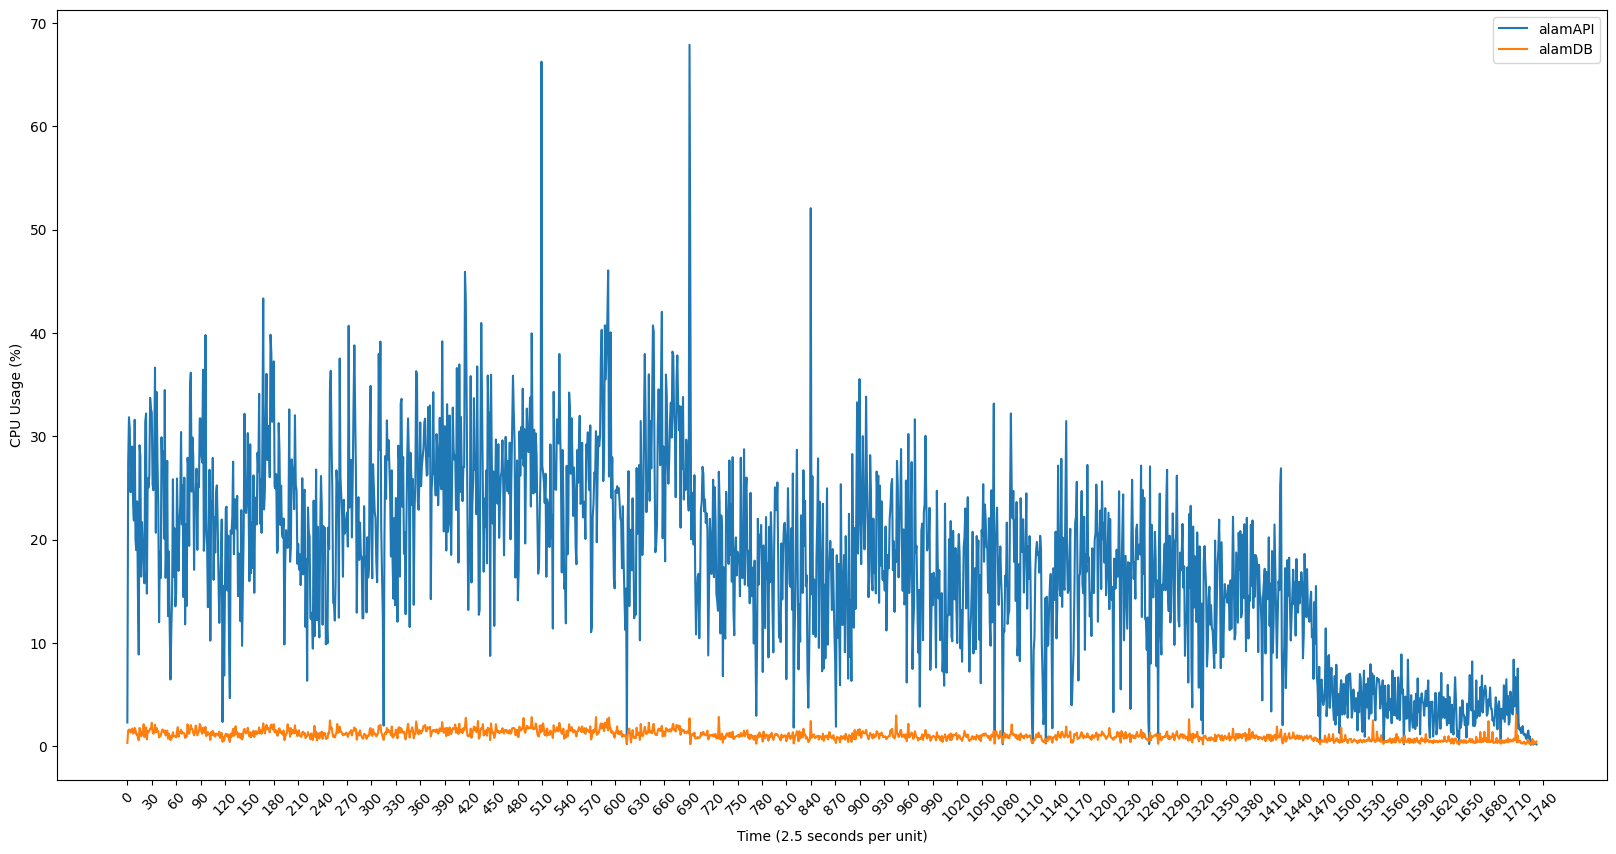
\includegraphics[width=1\textwidth]{./assets/Chapter_4/buy_sell/cpu_util.png}
    \caption{Deployment Load CPU Utilization of alamAPI and alamDB Over Time}
    \label{fig:cpu_util_onload}
\end{figure}
\FloatBarrier

\begin{figure}[ht]
    \centering
    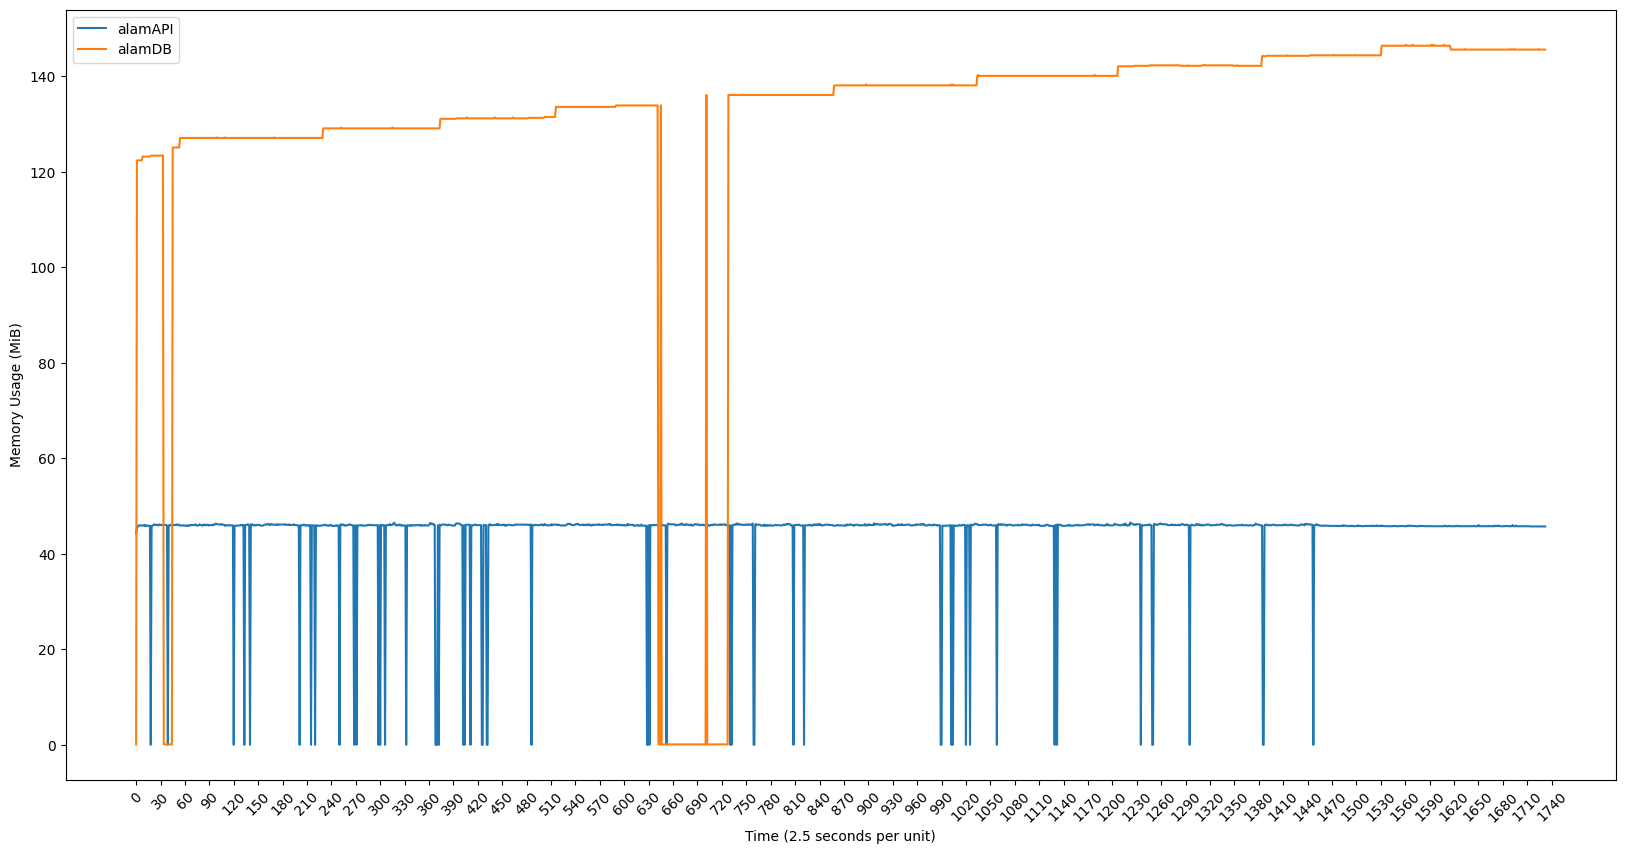
\includegraphics[width=1\textwidth]{./assets/Chapter_4/buy_sell/memory_util.png}
    \caption{Deployment Load Memory Utilization of alamAPI and alamDB Over Time}
    \label{fig:memory_util_onload}
\end{figure}
\FloatBarrier

Based on the table and figures above, processing all requests consumes only 
17.73\% and 1.07\% of the CPU for alamAPI and alamDB, respectively. 
In terms of memory usage, they are 44.62 MiB and 129.27 MiB, respectively.
\\

Furthermore, at around 1740 time units, the CPU utilization for alamAPI 
was shown to be reduced. This is due to the fact that most tester 
applications have already completed processing all of the requests that 
they are programmed to run, reducing the load on the server by half.
\\
